% Tikz File 'example_convex_boustrophedon.tex'
\documentclass{standalone}
\usepackage{tikz}

\usetikzlibrary{shadows.blur}
\usetikzlibrary{shapes.symbols}

%==============================================================================%
% TiKz Templates
\tikzset{% 
	box/.style={very thick,blur shadow={shadow blur steps=5},fill=white}
}
\tikzset{% 
	covered_area/.style={fill=green,opacity=0.4}
}
%==============================================================================%

\begin{document}
	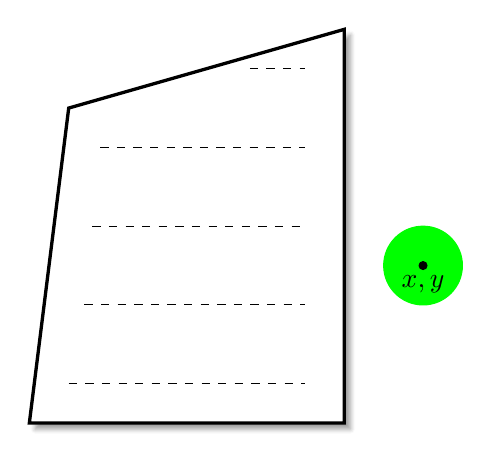
\begin{tikzpicture}[scale=1]
		\coordinate (p1) at (0,0);
		\coordinate (p2) at (4,0);
		\coordinate (p3) at (4,5);
		\coordinate (p4) at (0.5,4);

		\draw [box] (p1)--(p2)--(p3)--(p4)--cycle;

		\draw [fill,color=green] (5,2) circle [radius=0.5cm];
		\draw [fill] (5,2) circle [radius=0.05cm] node[below]{$x,y$};

		\draw [dashed] ([xshift=0.5cm,yshift=0.5cm]p1)--([xshift=-0.5cm,yshift=0.5cm]p2);
		\draw [dashed] ([xshift=0.7cm,yshift=1.5cm]p1)--([xshift=-0.5cm,yshift=1.5cm]p2);
		\draw [dashed] ([xshift=0.8cm,yshift=2.5cm]p1)--([xshift=-0.5cm,yshift=2.5cm]p2);
		\draw [dashed] ([xshift=0.9cm,yshift=3.5cm]p1)--([xshift=-0.5cm,yshift=3.5cm]p2);
		\draw [dashed] ([xshift=2.8cm,yshift=4.5cm]p1)--([xshift=-0.5cm,yshift=4.5cm]p2);

	\end{tikzpicture}
\end{document}